\subsection{Meteorologie}

Ich persönlich studiere Meteorologie auf Diplom und Physik auf Bachelor, habe daher selber Meteorologie als Nebenfach belegt. 
Im Folgenden möchte ich euch dieses Fach als Nebenfach vorstellen.\\
\fach{Meteorologie} ist ein sehr interessantes Fach, da es ziemlich viel mit Physik zu tun hat, das Thema aber einmal von einer anderen Perspektive angeht.
Es handelt sich dabei um eine noch sehr wenig erforschte Wissenschaft, die man aber im alltäglichen Leben leichter beobachten kann als einige andere Nebenfächer, die an der
Uni Frankfurt angeboten werden.\\
Nun aber zu den Inhalten und den Dingen, die ihr für dieses Fach leisten müsst.\\
Laut Bachelor - Prüfungsordnung können alle Module der bestehenden Bachelorordnung des Bachelorstudiengangs Meteorologie gewählt werden.\\
Ihr fangt mit dem Modul \Modul{EMet A} an.
Dieses umfasst die Vorlesungen \VL{Allgemeine Meteorologie} und \VL{Klimatologie} und gibt insgesamt 10 CP.\\
In der allgemeinen Meteorologie geht es z.B. um meteorologische Grundbegriffe, die Struktur der Atmosphäre und um Windgesetze. 
\begin{figure}[!t]
  \begin{center}
  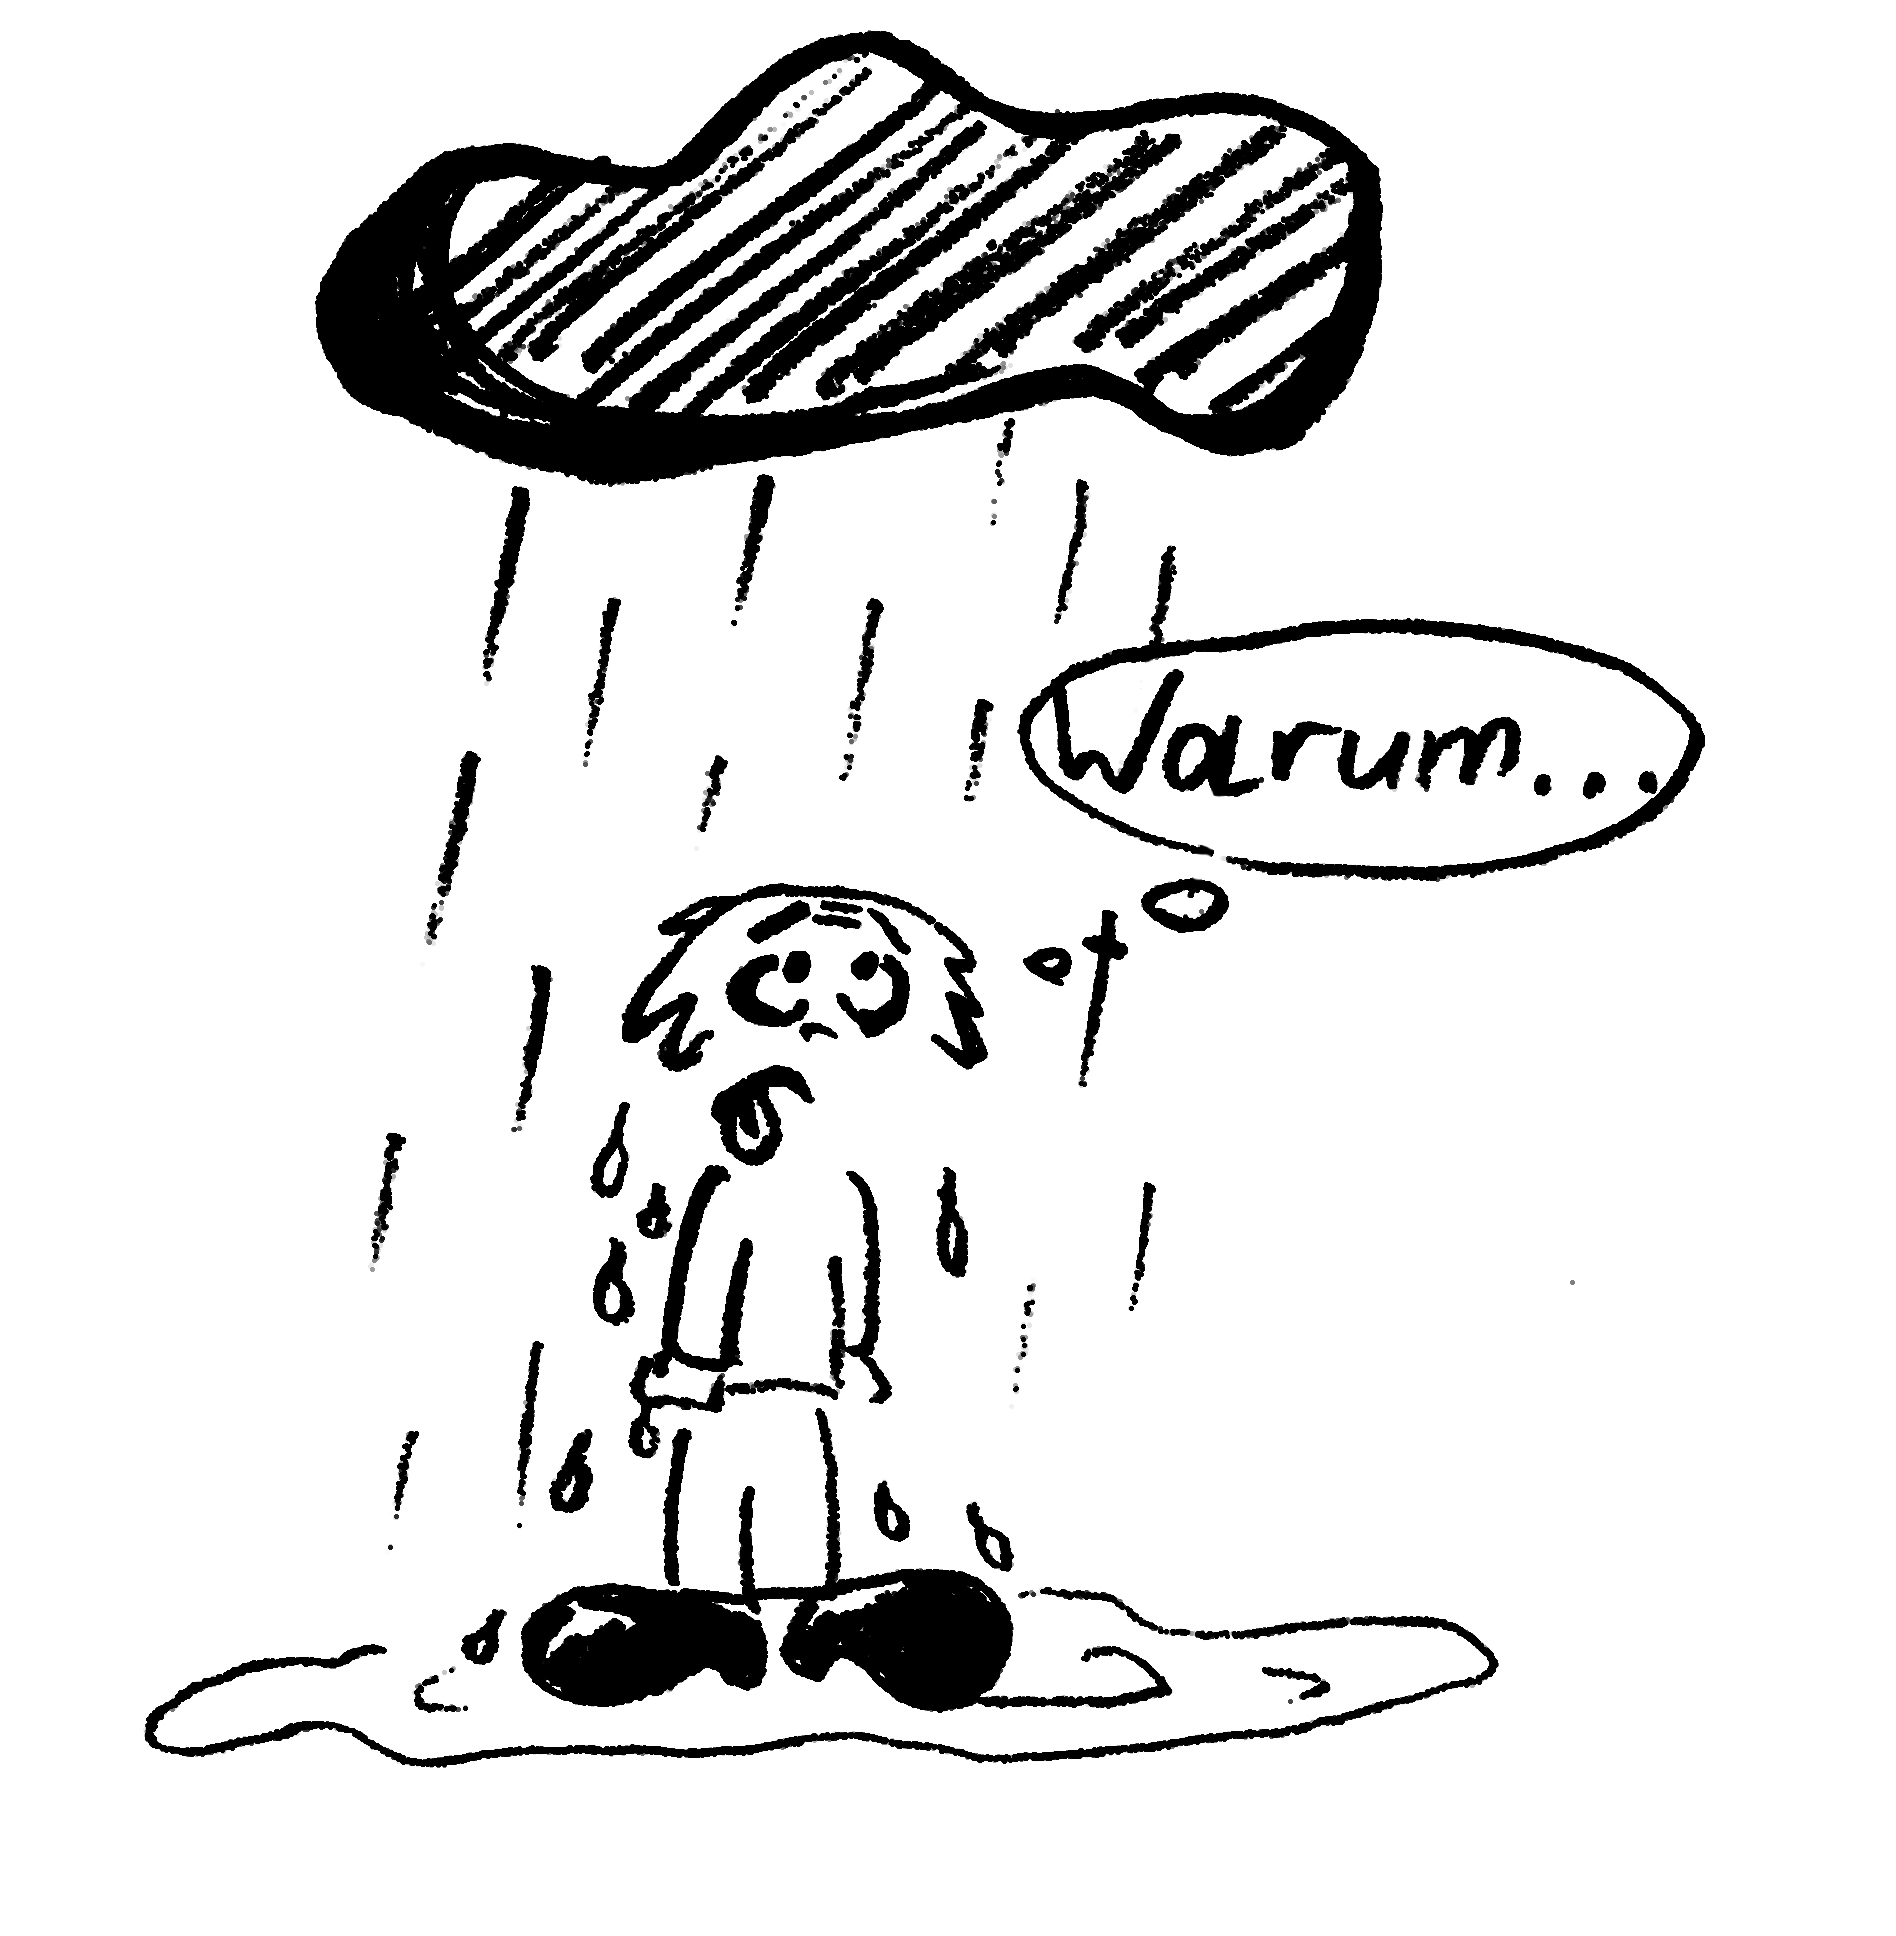
\includegraphics[width=.7\textwidth]{bilder/meteorologe.jpg}
\end{center}
\end{figure}

\pagebreak

Die Klimatologie betrachtet nicht kurzlebige Phänomene wie das Wetter, sondern lange Zeiträume von mindestens 30 Jahren.
Prof. Dr. Bodo Ahrens erklärt, wie man Klima "`macht"', also wie man es mit statistischen Methoden bestimmt und welche meteorologischen Größen dabei eine Rolle spielen.
\bigskip

Danach könnt ihr mit dem Modul \Modul{EMet B} weitermachen.
Dafür bekommt ihr auch 10 CP.
\\Das Modul umfasst eine Einführung in die Theoretische Meteorologie (\VL{Atmospheric Dynamics I} und \VL{II}).
\\Die Theoretische Meteorologie beschäftigt sich unter anderem mit der Kinematik des Windfeldes, der Newtonschen Mechanik und mit Thermodynamik.
\bigskip

Mit dem Modul \Modul{EMet A} könnt ihr direkt im Wintersemester anfangen.
Es sind keine Vorkenntnisse notwendig.
\von{Luisa}
